\chapter{Introduction
  \label{chap:introduction}}

%%% page numbering %%%
\pagenumbering{arabic}

\section{Origin of life and Origin of organic materials}
Life was born in "primordal soup", a warm sea containing high concentrations of organic materials synthesized by chemical evolution. But there are various hypothesis on how the soup was formed.
One hypothesis has been advocated that organic molecules synthesized in outer space 
was brought into the earth as a mechanism that organic matter accumulated on the earth.

A variety of organic molecules have been detected in outer space, and these are presumed 
to be formed by surface reaction or photochemical reaction on surface of icy mantle or grain 
in dense nebula such as dark nebula.
Solid particles eventually gather and grow, forming planetesimals and planets.

Many organic molecules including amino acids are found in meteorites.
A well-studied example of exogenous delivery of organic materials would
be the Murchison meteorite, which fell into Victoria, Australia, in 1969. 
Many authors have reported the detection of common amino acids such as glycine 
(the simplest amino acid; NH$_2$CH$_2$COOH), alanine, and glutamic acids \citep[e.g., ][]{Engel+Nagy1982}.

Moreover, glycine was also discovered from the comets. 
In 2006, NASA's Stardust spacecraft brought back samples from comet 81P/Wild 2 to the earth 
and \citet{Elsila+2009} claimed the detection of glycine in this comet.
In addition, glycine detection was reported in comet 67P/Churyumov-Gerasimenko by \citet{Altwegg+2016},
which contained molecules considered as precursors of glycine (e.g., methylamine and ethylamine).

As mentioned above, these organic molecules may be synthesized in outer space and then 
come to the earth with cosmic dust and meteorites.
Especially comets are thought to be formed far from the central star in the protoplanetary disk, 
and protoplanetary disk was formed by shrinking of interstellar molecular clouds. 
For this reason, it is inferred that the materials formed in the interstellar molecular cloud 
are kept in the comets.
Therefore, the presence of glycine in the comets suggests that glycine and other amino acids 
may exist in interstellar molecular clouds.

However, a certain detection of glycine in molecular clouds has not been reported, and
its origin is still unknown.
\citet{Kuan+2003} claimed the first detection of glycine, however, several follow-up observations 
denied the detection.
The emission Kuan et al. thought to be glycine was concluded to be acetone
\citep[e.g.,][]{Jones+2007}.

\newpage
\section{Star forming region}
Previous research has revealed that various organic molecules exist in the star formation regions so far. 
Here we introduce the celestial bodies that we focused on in this work.
\subsection{Orion Kleinmann-Low nebula}
\begin{figure}[ht]
  \hspace{-5cm}
  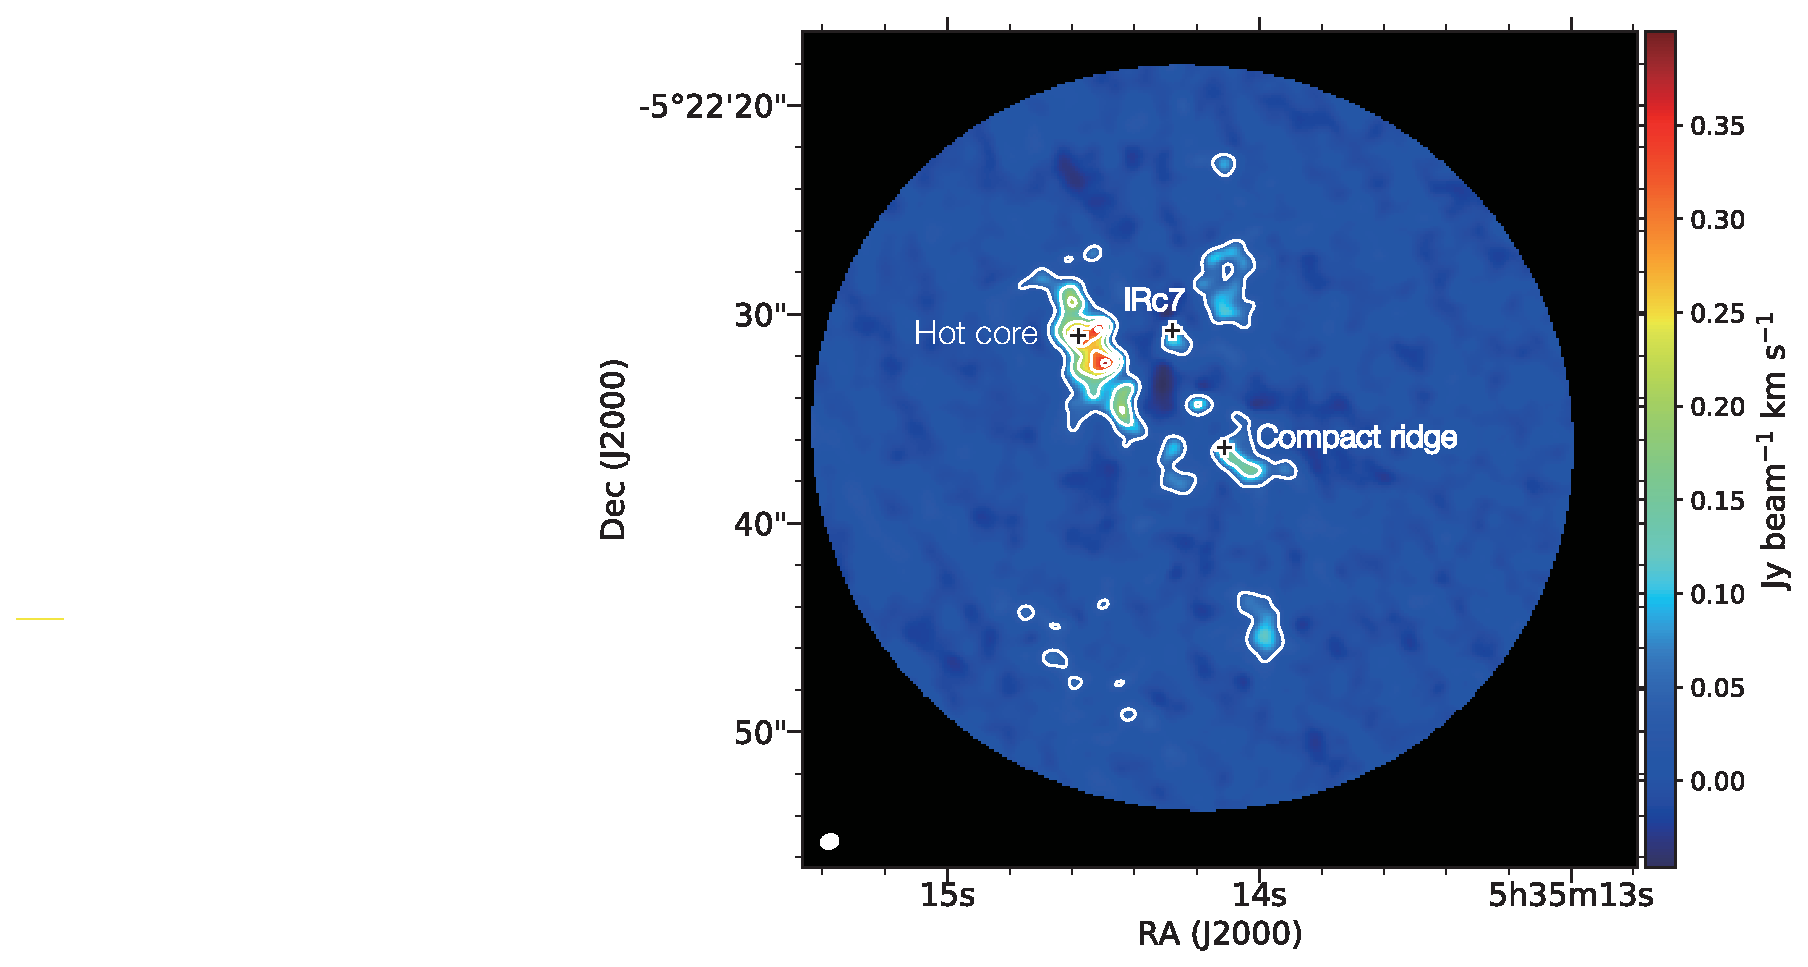
\includegraphics[width=18cm]{OrionKL/Orion_cnt.eps}
  \caption{Continuum emission map for band 6 data from \citet{Hirota+2015}. Synthesized beam size is indicated at the bottom-left corner. The contour levels are 10 \%, 30 \%, 50 \%, 70 \%, 90 \% of the peak intensity of 0.40 Jy/beam. Black crosses denote Hot core, IRc7, and Compact ridge}
  \label{fig:cont+2015}
  
\end{figure}

The Orion region hosts two well-studied star forming sites, Orion A and Orion B. 
Orion A is subdivided into four clouds (Orion Molecular Cloud 1-4, OMC) and 
OMC1 holds the Kleinmann-Low nebula (hereafter Orion-KL).

The Orion-KL is the nearest massive star-forming region, which is located approximately 
418 $\pm$ 6 pc away from the sun \citep{Kim+2008}. 
Its proximity and rich molecular composition make this region well suited for astrochemical study.
Since this region was discovered in 1967 \citep*{Kleinmann+1967},
numerous studies including line survey have been conducted so far \citep[e.g.,][]{Pagani+2017, Feng+2015, Gong+2015, Turner1991}.

In Orion-KL, several remarkable sources called Hot core and Compact ridge are known as regions where many organic molecules exist \citep{Blake+1987}. 
Hot core is known as a high-density (10$^6$ cm$^{-3}$) region with a warm ($\sim$ 150 K), compact ($<$ 0.05 pc) clump \citep{Zapata+2011}, and Compact ridge is also known to be a warm and dense region. 
Many previous studies have revealed that the chemical composition is different between these regions.
While many molecules containing nitrogen (e.g., NH$_3$, CH$_3$CN, etc.) are observed 
in Hot core, 
O-bearing species (e.g.,CH$_3$OH, CH$_3$OCH$_3$, etc.) are observed in Compact ridge \citep{Favre+2011a}.

\subsection{Low mass star-forming regions}
Chemical studies of low mass star-forming regions were relatively sparse before the 1990s.
The chemical compositions of low mass star-forming regions were studied using a few abundant
molecules such as NH$_2$, CS, and HC$_3$N because molecular emission is generally weaker in low mass star-forming regions than in high mass star-forming regions. 
However, with the development of observation equipment, the chemical composition of 
low mass star-forming regions has gradually become clear.

Here, two low mass Class 0 protostars are taken as an example.
\begin{enumerate}
  \item IRAS 16293-2422 \\
IRAS 16293-2422 (hereafter IRAS 16293) is a deeply embedded young stellar object located 
in the L1689 region in the eastern part of the $\rho$ Ophiuchus cloud \citep[at d = 120 pc][]{Loinard+2008}.
It is a multiple system consisting of sources A and B, whose projected separation is 5'' (600 au).

This object is a typical example of sources with many saturated molecules, called hot corino \citep{Cazaux+2003}.
Saturated COMs( Complex organic molecules; Species consisting of 6 atoms or more) such as 
CH$_3$OH, CH$_3$CN, HCOOCH$_3$, (CH$_3$)$_2$O, C$_2$H$_5$OH, and C$_2$H$_5$CN were found 
\citep{Blake+1994,vanDishoeck+1995,Cazaux+2003}.

After the start of ALMA operation, COMs survey has been actively conducted. 
\citep[e.g., The ALMA Protostellar Interferometric Line Survey (PILS)][]{Jorgensen+2016}

  \item L483 \\
L483 is a dark cloud in Aquila Rift, whose distance from the Sun is 200 pc \citep{Jorgensen+2002,Rice+2006}.
This cloud is associated with the infrared source IRAS 18148-0440,
which is known to be a Class 0 protostar \citep{Fuller+1995,Chapman+2013}.
As opposed to hot corino, carbon chain molecules \citep[e.g., CS, CCH. See][]{Hirota+2009,Hirota+2010}
 are detected in this source, and 
recently, detection of unsaturated species such as CNCN, NCCN, and NCO has been reported by single-dish observation \citep{Agndez+2018,Marcelino+2018}.
In addition, saturated organic molecules such as CH$_3$OH, HCOOCH$_3$ and HNCO are 
detected as in IRAS 16293 by the high resolution observation with the interferometer \citep{Oya+2018b}.
\end{enumerate}

\newpage
\section{Radio observation}
The radio observation has been established as one method of space observations 
since discovery of the first cosmic radio by Karl G. Jansky in the 1930's and the world's first radio telescope made by Grote Reber. 
It has also made great development with the progress of radar technology during World War II.
Since then, observations have been carried out at multiple wavelength (not only visible light and radio but also X-rays and infrared), 
and unveiling the wonders of the universe that can not be understood only by visible light.
However, because of the influence of atmospheric absorption, only visible light, radio waves and part of infrared radiation are observable from the ground.
In terms of radio observation, frequency below 20 MHz do not pass through the ionosphere, 
and at high frequencies they are easily absorbed by atmospheric oxygen and water vapor. 
For this reason, it is appropriate to install the radio telescope in places with high altitude and low water vapor. 

The characteristics of radio observation that are not in other wavelength are as follows.\begin{itemize}
\item Low energy\\
The temperature at which the peak of the blackbody radiation is located in the millimeter or the submillimeter wave range is about 10--50 K.
Temperature of molecular cloud cores where the protostar is born is typically as low as 10 K. 
Therefore, we can explore the formation process of primitive star and its evolution by radio observation. 
And also it is possible to observe molecular emission lines existing around the cores.

\item Long wavelength\\
Radio is hard to be absorbed by interstellar microparticles, and it is possible to observe deeply in molecular cloud cores.

\item Well-established interference technology\\
In a telescope called an interferometer, it is possible to obtain a high resolution by observing 
with multiple remote antennas and interfering radio waves. 
\end{itemize}

With the above characteristics, radio observation regarded as important tool in astronomy.

\subsection{ALMA}
Atacama Large Millimeter/submillimeter Array (ALMA) is a synthetic aperture radio telescope 
in the Atacama desert in Chile.
Atacama desert has  high clear-sky ratio (low annual rainfall of 100 mm or less) and 
high altitude (about 5000 m), so the amount of water vapor in the sky is small. 
We can observe radio waves from celestial bodies without being affected by atmospheric 
absorption as much as possible there.
Because of the wide flat ground, the antenna can be arranged in a wide range of 18.5 km, 
its resolution corresponds to one large telescope with the same diameter.

Although high resolution observation can be cited as an advantage of the interferometer, 
on the other hand, it is not very suitable for the weak line survey because of the difficulty in improving sensitivity with the sparse array. 
However, by combining a short baseline antenna group and a long baseline antenna group,
ALMA enabled simultaneous high sensitivity and high resolution observation. 
It is expected that even COMs that have not been detected in the past can be found by ALMA observations.

\begin{figure}[H]
  \centering
  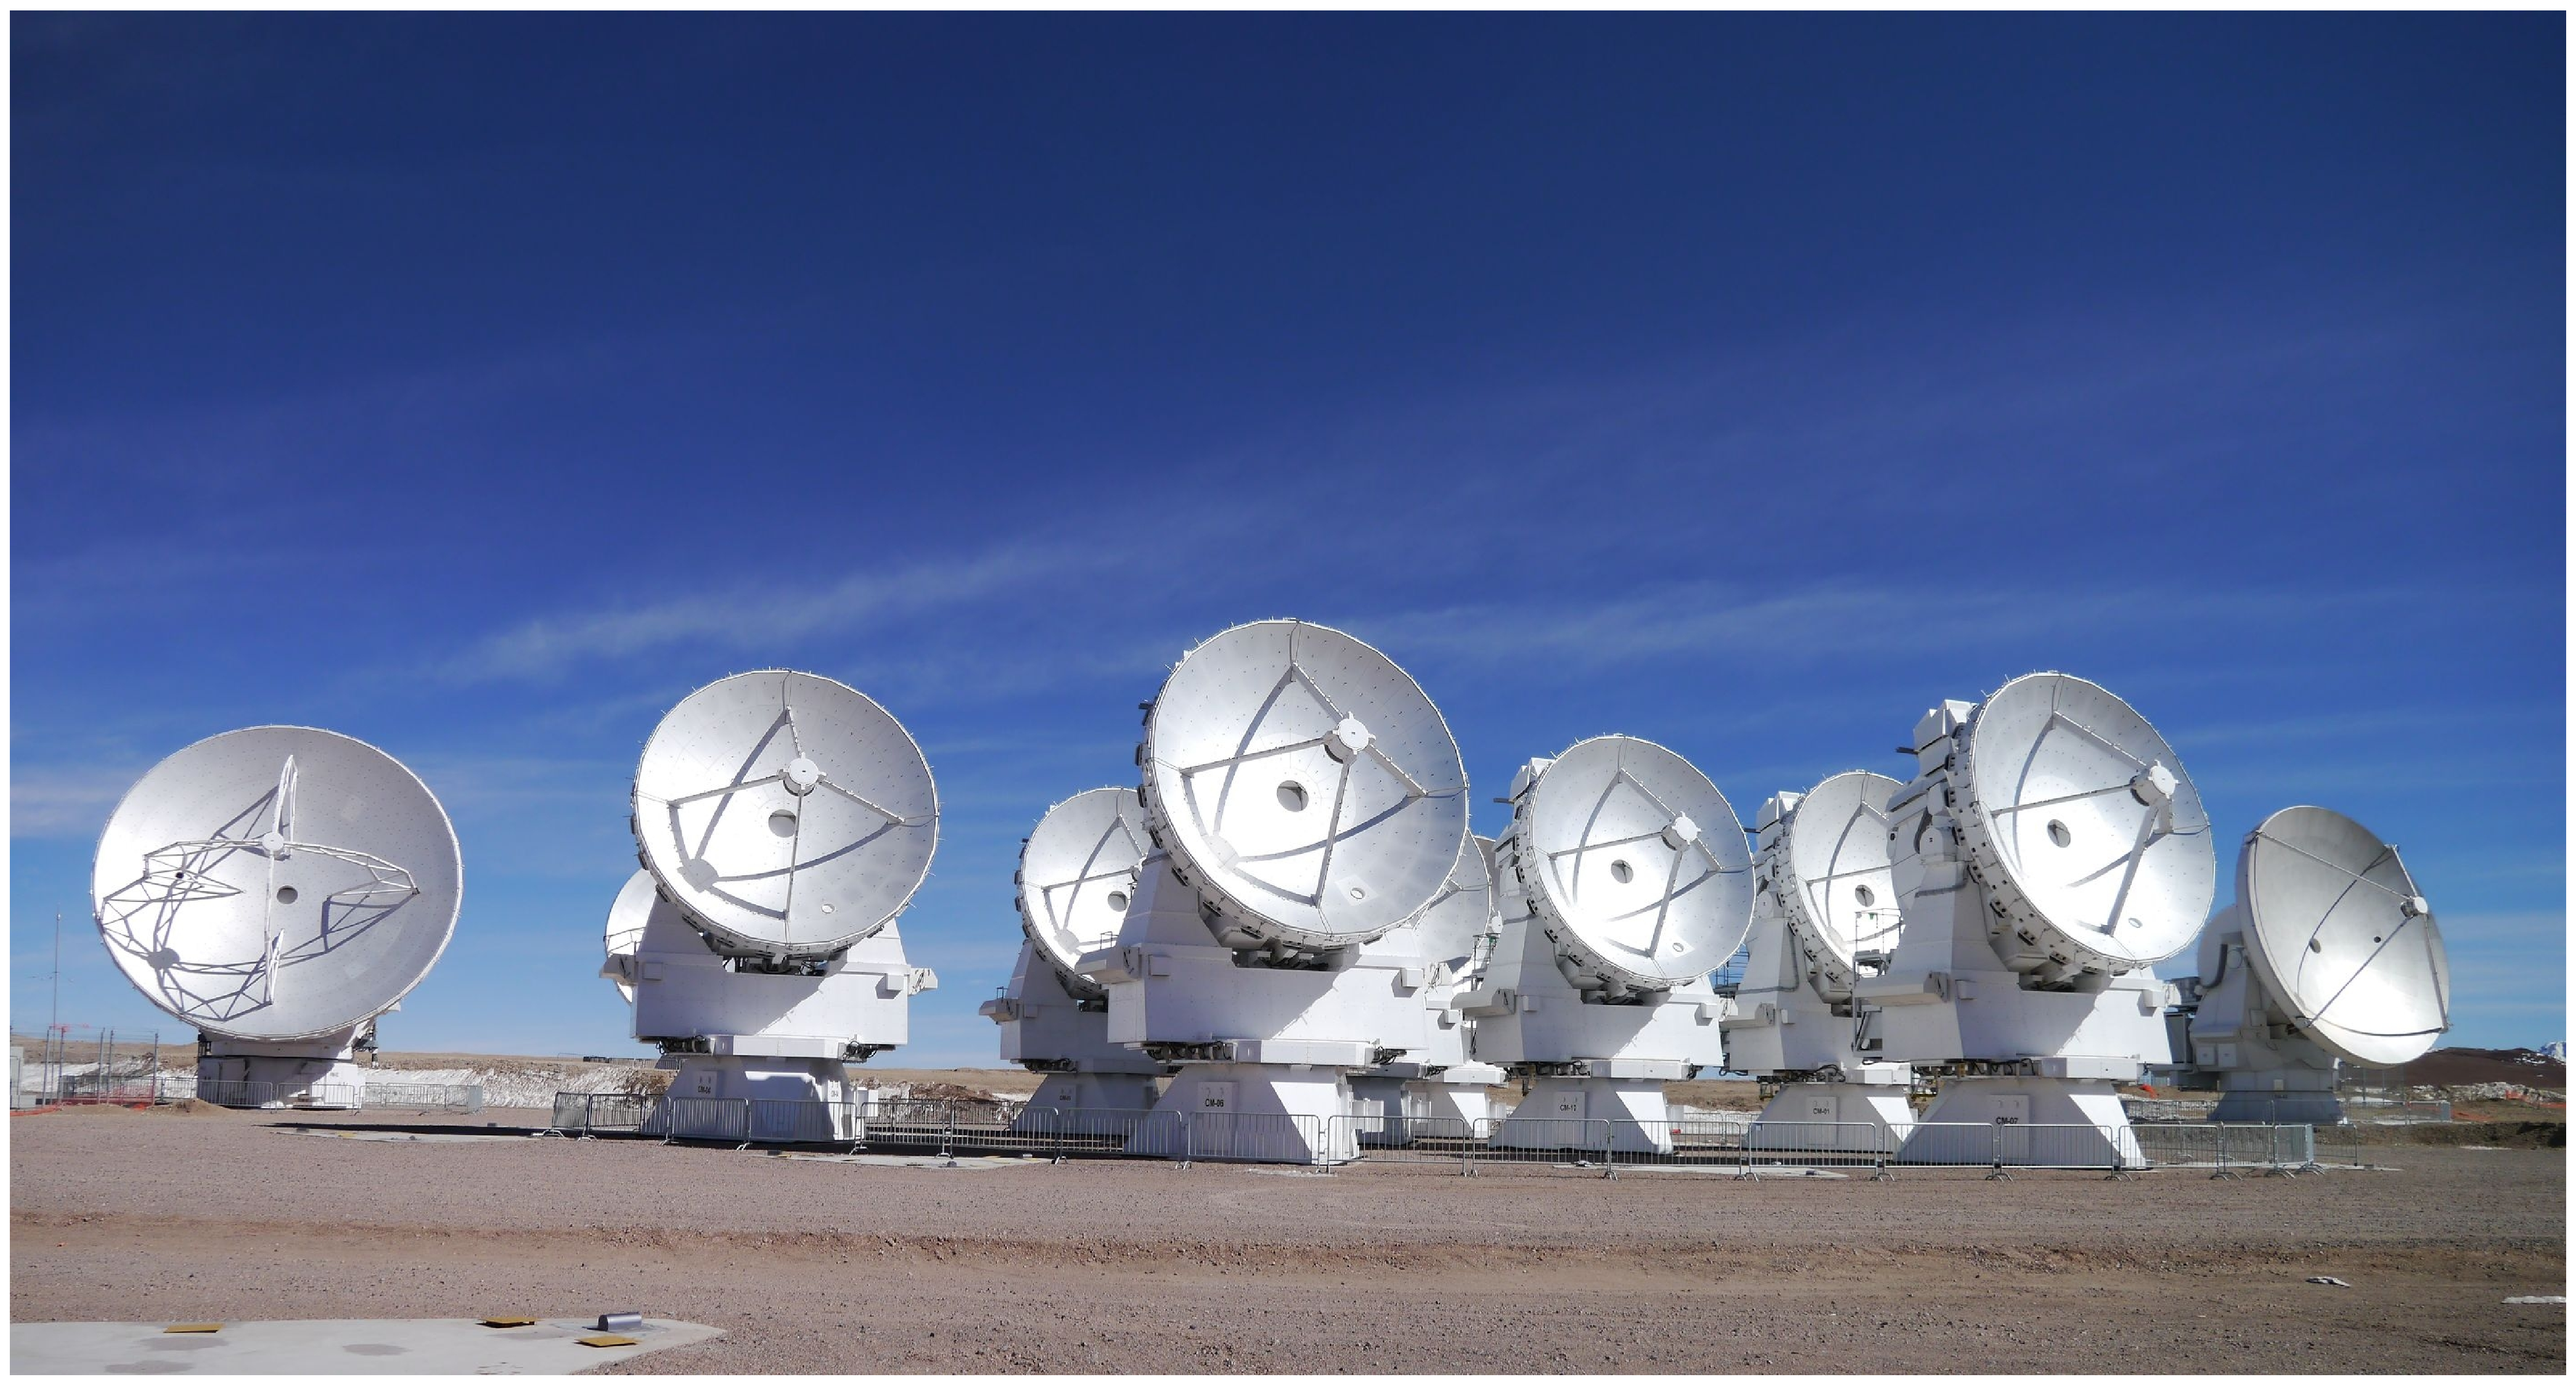
\includegraphics[width=0.7\textwidth]{ALMA.eps}
  \caption{Atacama Large Millimeter/submillimeter Array. Credit by ALMA (ESO/NAOJ/NRAO), R. Hills (ALMA)}
\end{figure}

\newpage
\section{CH$_3$NH$_2$, a precursor of glycine}
Methylamine (CH$_3$NH$_2$) is considered as a precursor of the simplest amino acid glycine. 
Recent experimental studies have shown several reaction pathways to forming
glycine in water containing ices starting from CH$_3$NH$_2$ and CO$_2$
subjected to high energy electrons \citep{Holtom+2005} or UV radiation \citep{Bossa+2009, Lee+2009}. Under similar conditions glycine can decompose to yield CH$_3$NH$_2$ and CO$_2$
\citep{Ehrenfreund+2001}. 

Interstellar CH$_3$NH$_2$ was first detected toward Sgr B2 at 3.5 cm \citep{Fourikis+1974} 
and at 3mm \citep{Kaifu+1974}. Recently, CH$_3$NH$_2$ has been detected 
in cometary samples of the Stardust mission \citep{Glavin+2008} and comet 67P/C-G \citep{Altwegg+2016, Altwegg+2017}.

However, in molecular clouds, 
a robust detection of CH$_3$NH$_2$ has been reported only for Sgr B2(N) \citep{Halfen+2013}  so far, 
while a variety of complex organic molecules have been detected by radio observations.
Although tentative detection in Orion-KL reported by \citet{Pagani+2017}, its physical properties 
such as distribution and temperature are still unclear.

\newpage
\section{Purpose of this work}
Since glycine has not been detected in the ISM, its precursors would be essential in
searching for good candidate sources for glycine surveys. 
Although CH$_3$NH$_2$  is a probable precursor, its detection has been reported only for one object. 
Since CO$_2$ exists in most of molecular clouds and CH$_3$NH$_2$ is a direct precursor
candidate to glycine, CH$_3$NH$_2$-rich sources will turn into promising glycine survey targets. 
Such studies would also accelerate the discussion regarding the exogenous delivery of 
prebiotic species to planets and connection between the Universe and life.
Therefore, in this study, we aim to detect CH$_3$NH$_2$ in the star-formation regions other than Sgr B2.

This paper is organized as follows. 
In Section 2, we present the observations and the data reduction.
In Sect. 3, we report distribution maps and spectrum  of several CH$_3$NH$_2$ candidate lines, 
and in Sect. 4 we discuss column density of CH$_3$NH$_2$ and predictable line contaminations.
Conclusions are summarized in Sect. 5.

